\section{Versioning et les environnements}\label{sec:versioning-environments}

Dans l'entreprise, les équipes de développement utilisent Git pour la gestion des versions et GitLab pour gérer le processus de développement.

Git est un système de gestion de version décentralisé largement utilisé dans le développement de logiciels. Il permet aux équipes de collaborer efficacement sur des projets en suivant les modifications apportées aux fichiers au fil du temps. Grâce à Git, les développeurs peuvent créer des branches pour travailler sur des fonctionnalités spécifiques ou des corrections de bugs sans perturber le code principal. Les commits, qui représentent des enregistrements de changements, sont la pierre angulaire de Git, permettant de garder une trace claire de l'évolution du code.

GitLab, quant à lui, est une plateforme de gestion de développement logiciel basée sur Git. Elle offre un environnement complet pour le cycle de vie du développement, de la planification à la surveillance. GitLab permet aux équipes de suivre les problèmes, de planifier les sprints, de gérer les demandes d'extraction et de créer des pipelines d'intégration continue pour automatiser les tests et le déploiement. En regroupant toutes ces fonctionnalités au même endroit, GitLab facilite la collaboration entre les membres de l'équipe et permet une gestion transparente et efficace des projets de développement.

Parmi ces nombreuses fonctionnalités, les équipes de DevOps et de développement n'utilisent cependant pas les fonctionnalités de gestion de projet et d'intégration continue/de livraison continue de GitLab, puisqu'elles utilisent Jira (comme nous l'avons vu dans la section précédente) et TeamCity (comme nous le verrons dans la section suivante) à ces fins. GitLab est donc principalement utilisé comme un hébergeur de dépôt de code et un outil de révision de code avec des fonctionnalités telles que les demandes de fusion (merge request).

La Figure~\ref{fig:versioning-and-environments} illustre les principes du versioning et les différents environnements utilisés pour héberger les différentes versions du code. La Table~\ref{tblr:environments} apporte quelques compléments d'information.

Du point de vue des versions et des environnements, le processus de développement entre deux éditions est le suivant. Avant la sortie publique de la nouvelle édition, il y a toujours une sortie interne. La sortie interne est créée par la fusion de la branche \mintinline{console}{develop} dans la branche \mintinline{console}{master} avec la balise \mintinline{console}{{numéro d'édition}.0}. Après cela, une nouvelle branche de \mintinline{console}{release} est créée à partir de la branche \mintinline{console}{master} avec le nom \mintinline{console}{release/{numéro d'édition}}. Cette nouvelle branche \mintinline{console}{release} n'est pas touchée avant la sortie publique.

Entre la sortie interne et la sortie publique, des correctifs urgents (\mintinline{console}{hotfix}) peuvent être apportés. Lorsque le développeur travaille sur un \mintinline{console}{hotfix}, il crée d'abord une branche à partir de l'ancienne branche \mintinline{console}{release} avec un nom \mintinline{console}{hotfix/{bogue}}, il y dépose ses modifications en travaillant dans son environnement sandbox développeur, puis il crée une demande de fusion pour réintégrer cette branche dans l'ancienne branche \mintinline{console}{release}. Lorsqu'une décision positive est prise concernant la sortie publique, l'ancienne branche \mintinline{console}{release} est fusionnée dans les branches \mintinline{console}{master} et \mintinline{console}{develop}, l'ancienne branche \mintinline{console}{release} est clôturée (archivée), la branche \mintinline{console}{master} est fusionnée dans la nouvelle branche \mintinline{console}{release}, puis la nouvelle branche \mintinline{console}{release} est fusionnée dans la branche \mintinline{console}{develop}, enfin la branche \mintinline{console}{master} est mise en production dans l'environnement de production avec la balise \mintinline{console}{{numéro d'édition}.1}. Pendant la période entre la sortie interne et la sortie publique, les développeurs peuvent travailler sur de nouvelles fonctionnalités, mais celles-ci ne seront pas intégrées dans l'édition actuelle, elles ne pourront l'être que dans la prochaine.

Après la sortie publique de la nouvelle édition, les développeurs commencent à travailler sur la prochaine édition. Lorsqu'ils travaillent sur des bogues, des correctifs (\mintinline{console}{fix}), ils créent une branche à partir de la branche \mintinline{console}{release} avec un nom \mintinline{console}{fix/{bogue}}, ils travaillent dans leur environnement sandbox, et lorsqu'ils ont terminé, ils créent une demande de fusion pour fusionner leur branche dans la branche \mintinline{console}{release}. Lorsqu'ils travaillent sur des fonctionnalités, cela se passe de la même manière, sauf qu'ils créent leur branche à partir de la branche \mintinline{console}{develop} avec un nom \mintinline{console}{feat/{fonctionnalité}} et bien sûr ils créent la demande de fusion pour fusionner leur branche dans la branche \mintinline{console}{develop}. Au cours de cette période, les corrections peuvent être fusionnées dans les branches \mintinline{console}{master} et \mintinline{console}{develop} et elles peuvent être mises en production si nécessaire à la fin des sprints ou même au milieu de ceux-ci. Dans ce cas, une nouvelle subversion est ajoutée au commit de fusion sous la forme d'une balise (\mintinline{console}{{numéro d'édition}.{numéro d'increment}}).

\begin{sidewaysfigure}
    \centering
    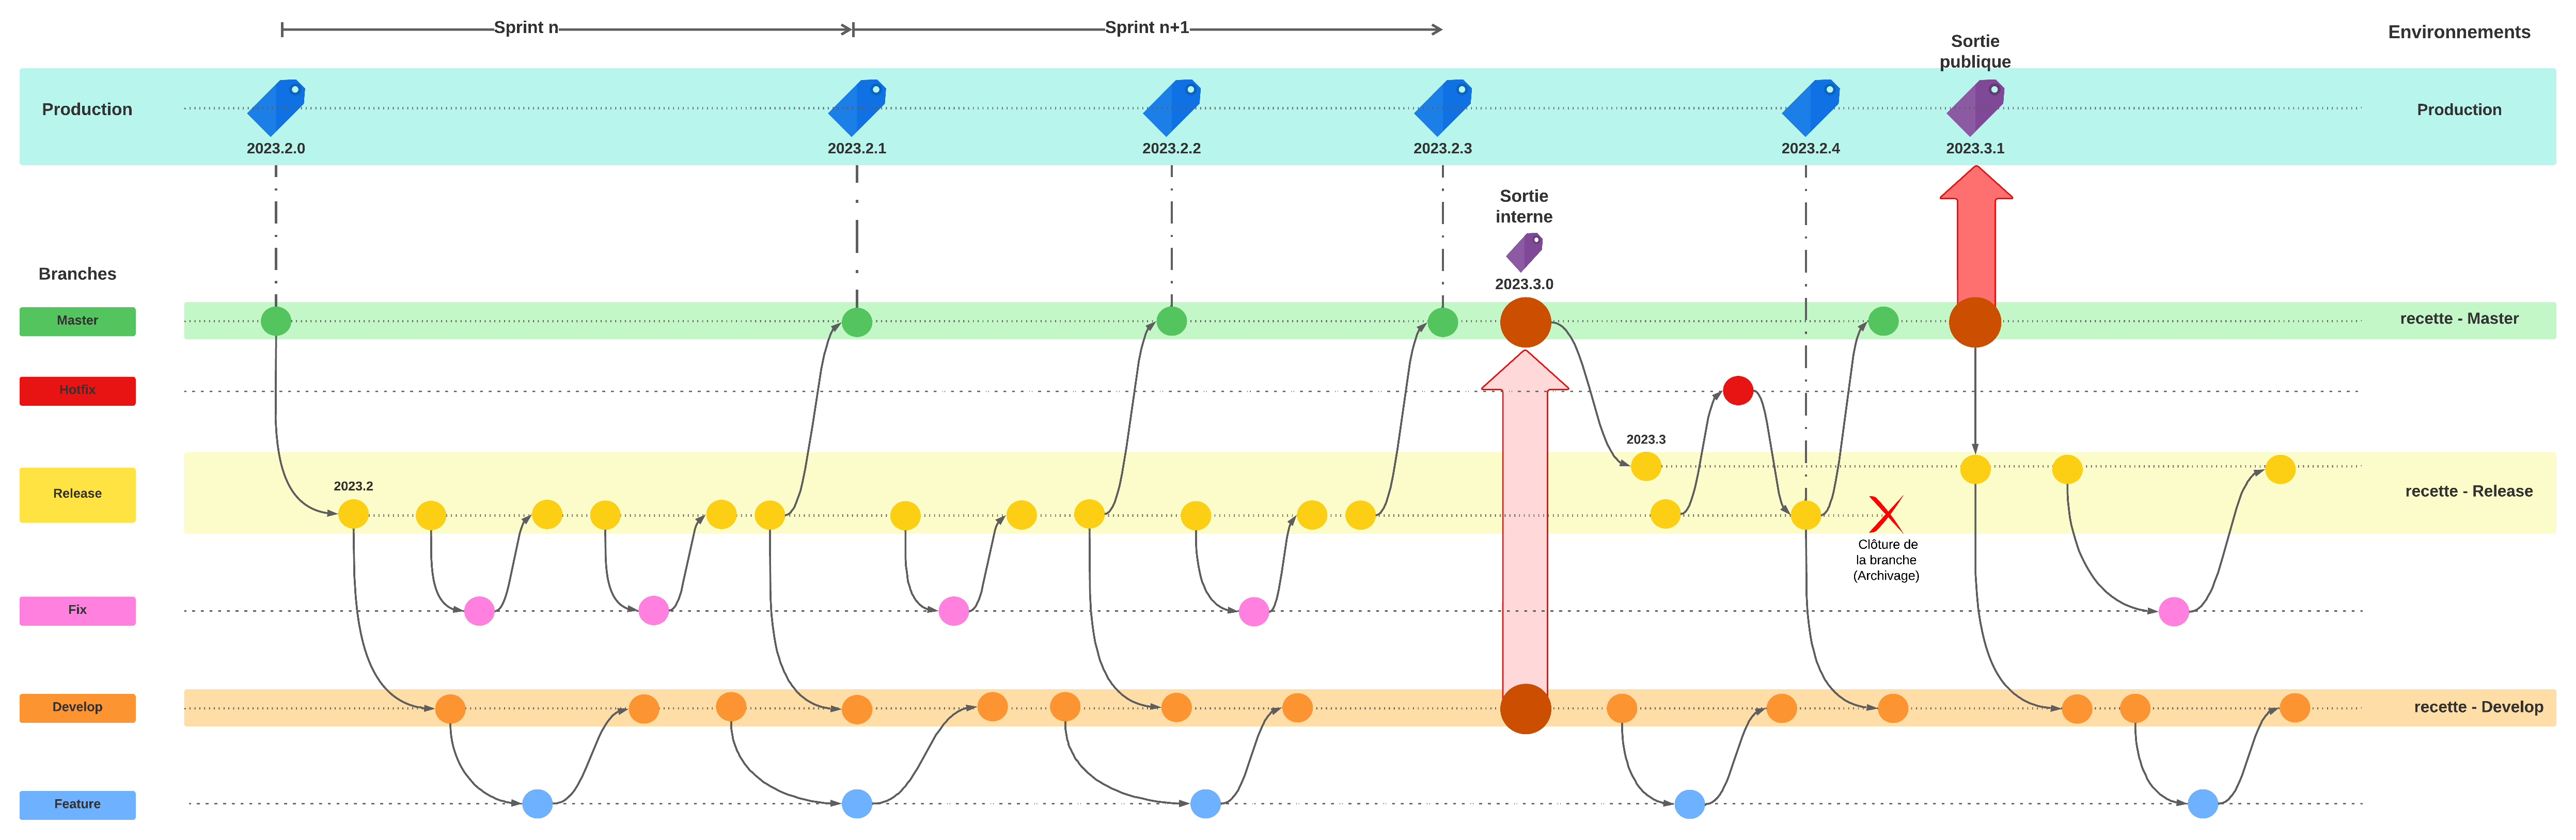
\includegraphics[width=\textwidth]{img/versioning-and-environments}
    \caption{Le schéma du versioning et les environnements.}
    \label{fig:versioning-and-environments}
\end{sidewaysfigure}

\begin{longtblr}[
    caption={Les caractéristiques des différents environnements.},
    label={tblr:environments}
    ]{
    hlines,vlines,
    rowspec={Q[m,font=\footnotesize\bfseries,gray9]*{5}{Q[m,font=\footnotesize]}}
    }
    Environnement    & {Pour quels                       \\ services} & Branches & {Type de \\ comits} & {Déploiement \\ TeamCity} \\
    {sandbox                                             \\ développeur} & Développeur & {feat/\\\{fonction-\\nalité\} \\ fix/\{bogue\} \\ hotfix/\{bogue\}} &  & -- \\
    recette-develop  & {Le PO vérifie                    \\ les fonction-\\nalités}                                & develop             & feat                                                         & Auto                                                                      \\
    recette-releases & {Le PO vérifie                    \\ les corrections}                                    & releases/édition    & fix, hotfix                                                          & Auto                                                                      \\
    recette-master   & {Autres                           \\ services                    \\ pour test \\ (direction, \\ marketing, \\ commerce \\ \dots)} & master              & {(env juste \\ avant la prod, \\ préproduction)}                     & {Manuel, \\ section master \\ dans TeamCity, \\ demande via \\ ticket MEP \\ à DevOps}     \\
    production       &                & tag & {Commit en \\ production \\ avec tag \\ \{numéro d'édtion\}.\\\{numéro \\ d'increment\}} & {Manuel, \\ section \\ production \\ dans TeamCity, \\ demande via \\ ticket MEP \\ à DevOps}
\end{longtblr}

A ce stade, il est important de noter que le processus expliqué ci-dessus ne concerne pas qu'un seul projet, mais que, puisqu'il y a plusieurs projets chez SuiviDeFlotte, il les concerne tous. Cela signifie que chaque projet dispose de ses propres branches de \mintinline{console}{develop}, de \mintinline{console}{release} et \mintinline{console}{master}, ainsi que de ses propres environnements. Pour donner une vue d'ensemble des différents projets, la Figure~\ref{fig:architecture} présente une image de l'architecture de projets chez SuiviDeFlotte et Beepiz.

\begin{figure}[h]
    \centering
    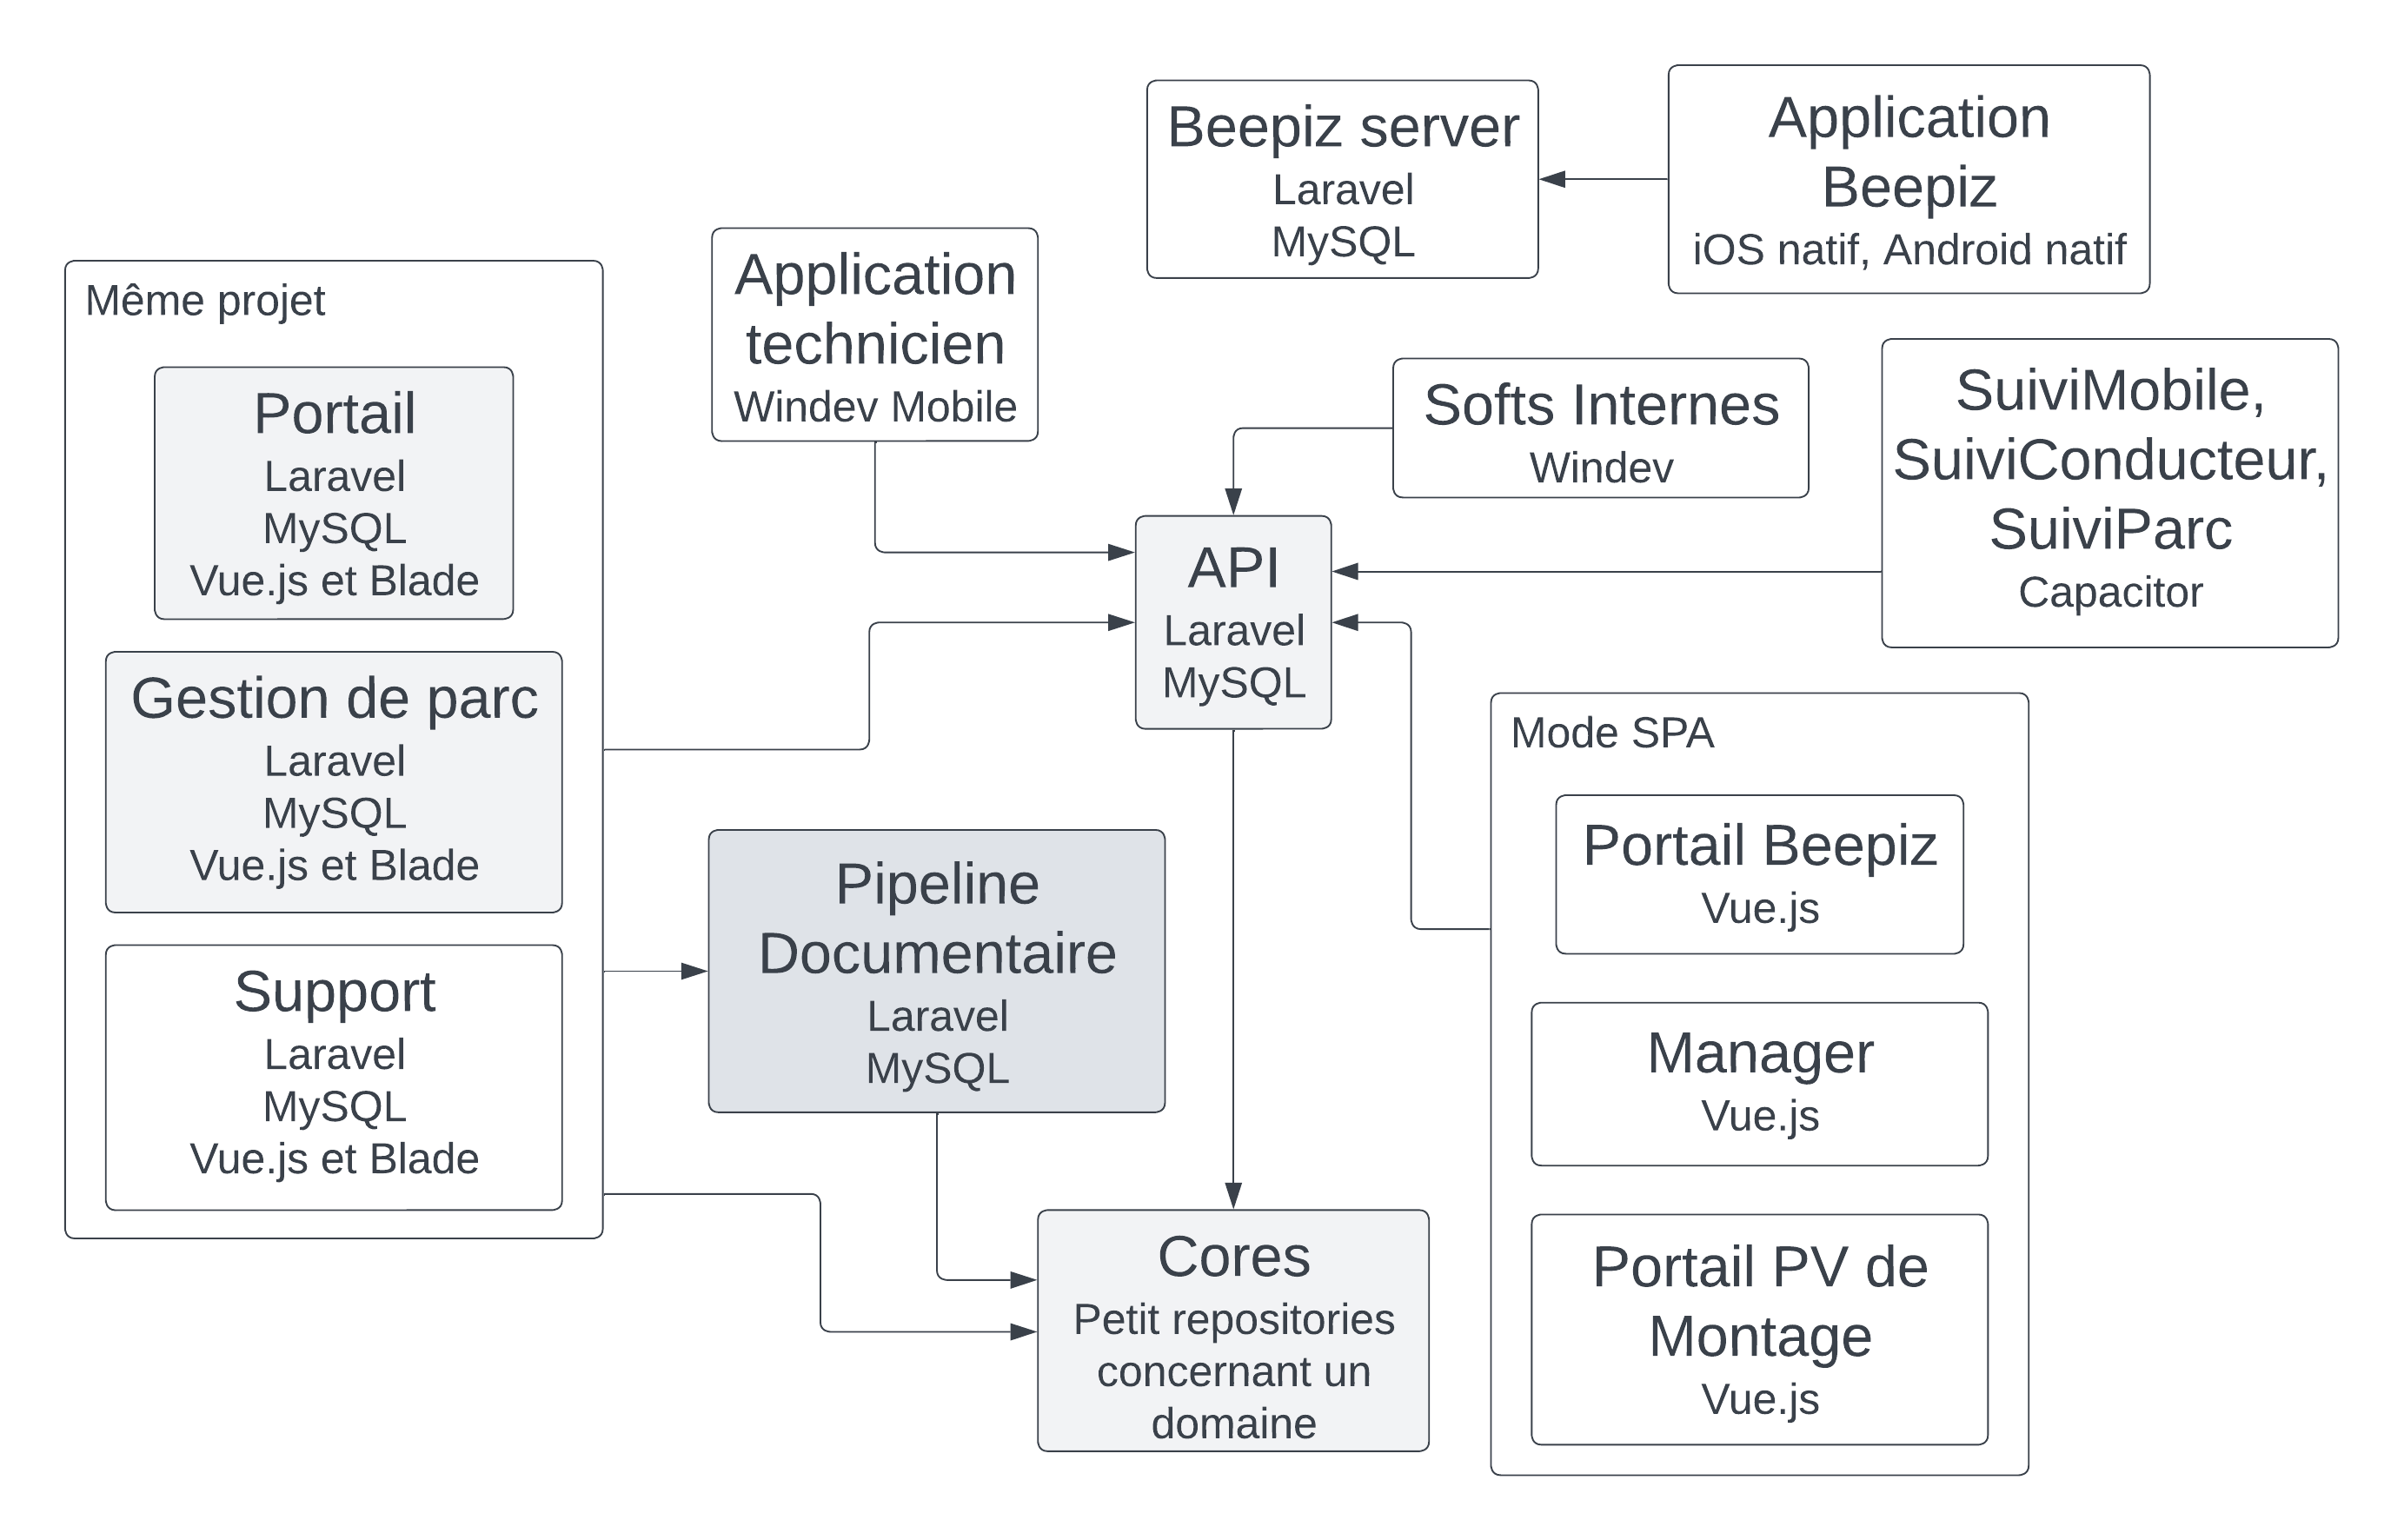
\includegraphics[width=\textwidth]{img/present-architecture}
    \caption{La vue d'ensemble des différents projets chez SuiviDeFlotte et Beepiz. Le projet principal sur lequel j'ai travaillé pendant mon alternance était le projet de Pipeline documentaire, mais j'ai également travaillé sur les projets colorés en gris clair.}
    \label{fig:architecture}
\end{figure}

Le nouveau projet sur lequel j'ai travaillé la plupart du temps pendant mon alternance est le projet Pipeline documentaire. Cependant, j'ai reçu de temps en temps des tickets de bogues provenant des projets Portail, Gestion de parc, API et Cores. De plus, j'ai travaillé sur une mission d'amélioration du frontend dans le projet Gestion de parc, qui était lié au projet Pipeline documentaire.

Le Portail, la Gestion du parc et le Support font partie du même projet Laravel qui est une application SaaS disponible pour les clients de SuiviDeFlotte. La partie Portail fournit les fonctionnalités de géolocalisation, la partie Gestion de parc fournit les fonctionnalités de gestion de parc comme son nom l'indique et la partie Support aide l'équipe de support dans son travail. L'API est un projet Laravel backend central qui fournit des données à d'autres projets à partir de la base de données. Le projet Cores implique un grand nombre de paquets PHP relativement petits qui sont stockés dans un dépôt de paquets privé créé par Satis.\footnote{Satis est un outil qui permet aux développeurs PHP de créer un dépôt de paquets privé pour les dépendances de leurs projets. Il offre un contrôle accru sur la distribution des paquets, une sécurité améliorée et des installations de paquets plus rapides, en créant un registre Composer statique qui peut être hébergé n'importe où (même via Docker, localement). Disponible sur \url{https://github.com/composer/satis}} Ces paquets contiennent des fonctionnalités communes qui peuvent être utiles dans plusieurs autres projets. Cependant, lorsque nous avons commencé à travailler sur le projet de Pipeline documentaire, nous avons commencé à travailler sur leur refactorisation et au cours de ce processus, nous avons créé un nouveau paquet (\mintinline{console}{core-redesing-share}) avec du code refactorisé provenant d'autres paquets et qui n'est pas encore utilisé, mais seulement par le Pipeline documentaire pour le moment.